\documentclass[a4paper,11pt]{article}
\usepackage[utf8]{inputenc}\usepackage[T1]{fontenc}
\usepackage[english]{babel}\usepackage{lmodern}\usepackage{microtype}
\usepackage{amsmath,amssymb}\usepackage{geometry}
\geometry{a4paper,left=2.2cm,right=2.2cm,top=2.0cm,bottom=2.0cm}
\usepackage{booktabs,array}\usepackage{xcolor}
\definecolor{bokug}{RGB}{0,135,60}\usepackage{tikz}
\usetikzlibrary{arrows.meta,calc}
\usepackage{fancyhdr}\pagestyle{fancy}
\renewcommand{\headrulewidth}{0.4pt}
\usepackage{enumitem}\setlength{\parindent}{0pt}\setlength{\parskip}{4pt}

\begin{document}
\fancyhead[L]{\small VU Mechanik – LAWI 100515 (PI)}\fancyhead[R]{\small SS 2026}\fancyfoot[C]{\thepage}
\begin{center}{\large\bfseries\color{bokug}University of Natural Resources and Life Sciences, Vienna (BOKU)}\\[2pt]{\large\bfseries VU Mechanik – LAWI 100515 (PI)}\\[4pt]Exam \textbf{Group A} \hfill Date: 26.06.2026\\[2pt]\rule{\linewidth}{0.4pt}\end{center}

\begin{center}\textbf{\large Model solution}\end{center}
\begin{center}
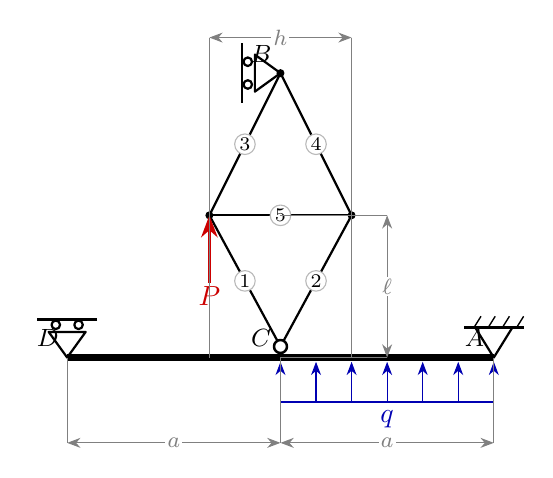
\begin{tikzpicture}[scale=0.903,>=Stealth,line join=round]
  \coordinate (P0) at (0.000,0.000);
  \coordinate (P1) at (-3.000,0.000);
  \coordinate (P2) at (-6.000,0.000);
  \coordinate (TO1) at (-4.000,2.000);
  \coordinate (TU0) at (-2.000,2.000);
  \coordinate (TO2) at (-3.000,4.000);
  \coordinate (CPIN) at (-3.000,0.155);
  \draw[thick] (CPIN) -- (TO1);
  \draw[thick] (CPIN) -- (TU0);
  \draw[thick] (TO1) -- (TO2);
  \draw[thick] (TU0) -- (TO2);
  \draw[thick] (TO1) -- (TU0);
  \draw[line width=2.2pt] (P0) -- (P1);
  \draw[line width=2.2pt] (P1) -- (P2);
  \fill (TO1) circle (1.6pt);
  \fill (TU0) circle (1.6pt);
  \fill (TO2) circle (1.6pt);
  \draw[fill=white,line width=0.9pt] (CPIN) circle (2.6pt);
  \draw[thick] (0.000,0.000) -- (0.260,0.420) -- (-0.260,0.420) -- cycle;
  \draw[line width=1pt] (0.420,0.420) -- (-0.420,0.420);
  \draw[line width=0.5pt] (0.320,0.420) -- (0.420,0.580);
  \draw[line width=0.5pt] (0.120,0.420) -- (0.220,0.580);
  \draw[line width=0.5pt] (-0.080,0.420) -- (0.020,0.580);
  \draw[line width=0.5pt] (-0.280,0.420) -- (-0.180,0.580);
  \draw[thick] (-6.000,0.000) -- (-5.740,0.360) -- (-6.260,0.360) -- cycle;
  \draw[thick] (-5.840,0.460) circle (0.06) (-6.160,0.460) circle (0.06);
  \draw[line width=1pt] (-5.580,0.540) -- (-6.420,0.540);
  \draw[thick] (-3.000,4.000) -- (-3.360,4.260) -- (-3.360,3.740) -- cycle;
  \draw[thick] (-3.460,4.160) circle (0.06) (-3.460,3.840) circle (0.06);
  \draw[line width=1pt] (-3.540,4.420) -- (-3.540,3.580);
  \node[circle,fill=white,draw=gray!55,inner sep=0.5pt,font=\scriptsize] at (-3.500,1.078) {1};
  \node[circle,fill=white,draw=gray!55,inner sep=0.5pt,font=\scriptsize] at (-2.500,1.078) {2};
  \node[circle,fill=white,draw=gray!55,inner sep=0.5pt,font=\scriptsize] at (-3.500,3.000) {3};
  \node[circle,fill=white,draw=gray!55,inner sep=0.5pt,font=\scriptsize] at (-2.500,3.000) {4};
  \node[circle,fill=white,draw=gray!55,inner sep=0.5pt,font=\scriptsize] at (-3.000,2.000) {5};
  \draw[->,blue!70!black] (0.000,-0.620) -- (0.000,-0.060);
  \draw[->,blue!70!black] (-0.500,-0.620) -- (-0.500,-0.060);
  \draw[->,blue!70!black] (-1.000,-0.620) -- (-1.000,-0.060);
  \draw[->,blue!70!black] (-1.500,-0.620) -- (-1.500,-0.060);
  \draw[->,blue!70!black] (-2.000,-0.620) -- (-2.000,-0.060);
  \draw[->,blue!70!black] (-2.500,-0.620) -- (-2.500,-0.060);
  \draw[->,blue!70!black] (-3.000,-0.620) -- (-3.000,-0.060);
  \draw[blue!70!black,thick] (0.000,-0.620) -- (-3.000,-0.620);
  \node[blue!70!black] at (-1.500,-0.870) {$q$};
  \draw[->,red!80!black,line width=1.1pt] (-4.000,1.050) -- (-4.000,2.000);
  \node[red!80!black] at (-4.000,0.870) {$P$};
  \draw[thin,gray] (0.000,0.000) -- (0.000,-1.200);
  \draw[thin,gray] (-3.000,0.000) -- (-3.000,-1.200);
  \draw[<->,gray] (0.000,-1.200) -- (-3.000,-1.200) node[midway,fill=white,inner sep=0.8pt,font=\footnotesize]{$a$};
  \draw[thin,gray] (-3.000,0.000) -- (-3.000,-1.200);
  \draw[thin,gray] (-6.000,0.000) -- (-6.000,-1.200);
  \draw[<->,gray] (-3.000,-1.200) -- (-6.000,-1.200) node[midway,fill=white,inner sep=0.8pt,font=\footnotesize]{$a$};
  \draw[thin,gray] (-3.000,0.000) -- (-1.500,0.000);
  \draw[thin,gray] (-3.000,2.000) -- (-1.500,2.000);
  \draw[<->,gray] (-1.500,0.000) -- (-1.500,2.000) node[midway,fill=white,inner sep=0.8pt,font=\footnotesize]{$\ell$};
  \draw[thin,gray] (-4.000,0.000) -- (-4.000,4.500);
  \draw[thin,gray] (-2.000,0.000) -- (-2.000,4.500);
  \draw[<->,gray] (-4.000,4.500) -- (-2.000,4.500) node[midway,fill=white,inner sep=0.8pt,font=\footnotesize]{$h$};
  \node[font=\small] at (0.000,0.000) [xshift=-7pt,yshift=7pt] {$A$};
  \node[font=\small] at (-3.000,0.000) [xshift=-7pt,yshift=7pt] {$C$};
  \node[font=\small] at (-6.000,0.000) [xshift=-7pt,yshift=7pt] {$D$};
  \node[font=\small] at (-3.000,4.000) [xshift=-7pt,yshift=7pt] {$B$};
\end{tikzpicture}
\end{center}
\par\medskip\textbf{1.\ Static determinacy}\par Counting criterion $n=3k-(a+z)$ (bodies $k$, reactions $a$, interaction forces $z$):
\[ n=3k-(a+z)=3\cdot2-(4+2)=0\ \Rightarrow\ \text{statically determinate} \]
\par\medskip\textbf{2.\ Support reactions and hinge forces}\par
$A:\ R_x=3.75,\ R_y=-12$\quad $D:\ R_x=0,\ R_y=-9$\quad $B:\ R_x=-3.75,\ R_y=0$\par $C:\ H_x=-3.75,\ H_y=15$
\par\medskip\textbf{3.\ Truss member forces}\par
\begin{center}\renewcommand{\arraystretch}{1.1}\begin{tabular}{c r l}
\toprule
Member & Force $S$ [kN] & Type \\
\midrule
  1 & 12.58 & tension \\
  2 & 4.19 & tension \\
  3 & -4.19 & compression \\
  4 & 4.19 & tension \\
  5 & -3.75 & compression \\
\bottomrule
\end{tabular}\end{center}
\begin{center}
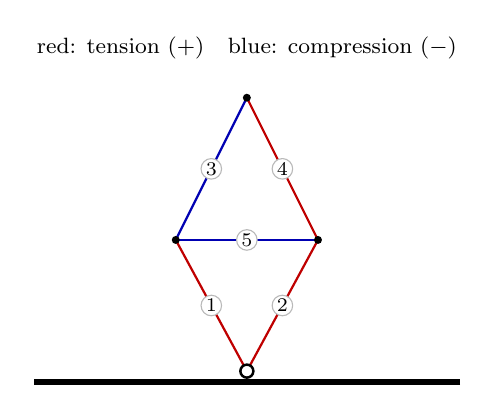
\begin{tikzpicture}[scale=0.903,>=Stealth,line join=round]
  \coordinate (P0) at (0.000,0.000);
  \coordinate (P1) at (-3.000,0.000);
  \coordinate (P2) at (-6.000,0.000);
  \coordinate (TO1) at (-4.000,2.000);
  \coordinate (TU0) at (-2.000,2.000);
  \coordinate (TO2) at (-3.000,4.000);
  \coordinate (CPIN) at (-3.000,0.155);
  \draw[thick,red!75!black] (CPIN) -- (TO1);
  \draw[thick,red!75!black] (CPIN) -- (TU0);
  \draw[thick,blue!70!black] (TO1) -- (TO2);
  \draw[thick,red!75!black] (TU0) -- (TO2);
  \draw[thick,blue!70!black] (TO1) -- (TU0);
  \draw[line width=2pt] (P0) -- (P1);
  \draw[line width=2pt] (P1) -- (P2);
  \fill (TO1) circle (1.6pt);
  \fill (TU0) circle (1.6pt);
  \fill (TO2) circle (1.6pt);
  \draw[fill=white,line width=0.9pt] (CPIN) circle (2.6pt);
  \node[circle,fill=white,draw=gray!55,inner sep=0.5pt,font=\scriptsize] at (-3.500,1.078) {1};
  \node[circle,fill=white,draw=gray!55,inner sep=0.5pt,font=\scriptsize] at (-2.500,1.078) {2};
  \node[circle,fill=white,draw=gray!55,inner sep=0.5pt,font=\scriptsize] at (-3.500,3.000) {3};
  \node[circle,fill=white,draw=gray!55,inner sep=0.5pt,font=\scriptsize] at (-2.500,3.000) {4};
  \node[circle,fill=white,draw=gray!55,inner sep=0.5pt,font=\scriptsize] at (-3.000,2.000) {5};
  \node[font=\footnotesize] at (-3.00,4.70) {red: tension $(+)$\quad blue: compression $(-)$};
\end{tikzpicture}
\end{center}
\par\medskip\textbf{4.\ Section-force diagrams of the beams}\par
\begin{center}
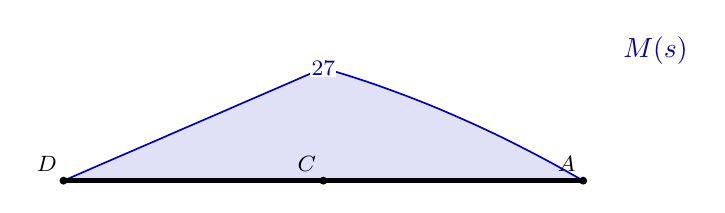
\begin{tikzpicture}[scale=1.100,line join=round]
  \filldraw[fill=blue!70!black!12,draw=blue!70!black,semithick] (0.000,0.000) -- (-0.125,0.071) -- (-0.250,0.141) -- (-0.375,0.210) -- (-0.500,0.277) -- (-0.625,0.342) -- (-0.750,0.406) -- (-0.875,0.469) -- (-1.000,0.530) -- (-1.125,0.589) -- (-1.250,0.647) -- (-1.375,0.703) -- (-1.500,0.758) -- (-1.625,0.812) -- (-1.750,0.864) -- (-1.875,0.914) -- (-2.000,0.963) -- (-2.125,1.010) -- (-2.250,1.056) -- (-2.375,1.101) -- (-2.500,1.144) -- (-2.625,1.185) -- (-2.750,1.225) -- (-2.875,1.263) -- (-3.000,1.300) -- (-3.000,1.300) -- (-3.125,1.246) -- (-3.250,1.192) -- (-3.375,1.137) -- (-3.500,1.083) -- (-3.625,1.029) -- (-3.750,0.975) -- (-3.875,0.921) -- (-4.000,0.867) -- (-4.125,0.812) -- (-4.250,0.758) -- (-4.375,0.704) -- (-4.500,0.650) -- (-4.625,0.596) -- (-4.750,0.542) -- (-4.875,0.487) -- (-5.000,0.433) -- (-5.125,0.379) -- (-5.250,0.325) -- (-5.375,0.271) -- (-5.500,0.217) -- (-5.625,0.163) -- (-5.750,0.108) -- (-5.875,0.054) -- (-6.000,0.000) -- (-6.000,0.000) -- (-5.875,0.000) -- (-5.750,0.000) -- (-5.625,0.000) -- (-5.500,0.000) -- (-5.375,0.000) -- (-5.250,0.000) -- (-5.125,0.000) -- (-5.000,0.000) -- (-4.875,0.000) -- (-4.750,0.000) -- (-4.625,0.000) -- (-4.500,0.000) -- (-4.375,0.000) -- (-4.250,0.000) -- (-4.125,0.000) -- (-4.000,0.000) -- (-3.875,0.000) -- (-3.750,0.000) -- (-3.625,0.000) -- (-3.500,0.000) -- (-3.375,0.000) -- (-3.250,0.000) -- (-3.125,0.000) -- (-3.000,0.000) -- (-3.000,0.000) -- (-2.875,0.000) -- (-2.750,0.000) -- (-2.625,0.000) -- (-2.500,0.000) -- (-2.375,0.000) -- (-2.250,0.000) -- (-2.125,0.000) -- (-2.000,0.000) -- (-1.875,0.000) -- (-1.750,0.000) -- (-1.625,0.000) -- (-1.500,0.000) -- (-1.375,0.000) -- (-1.250,0.000) -- (-1.125,0.000) -- (-1.000,0.000) -- (-0.875,0.000) -- (-0.750,0.000) -- (-0.625,0.000) -- (-0.500,0.000) -- (-0.375,0.000) -- (-0.250,0.000) -- (-0.125,0.000) -- (0.000,0.000) -- cycle;
  \draw[line width=1.6pt] (0.000,0.000) -- (-3.000,0.000) -- (-6.000,0.000);
  \node[blue!70!black,font=\footnotesize,fill=white,inner sep=0.5pt] at (-3.000,1.300) {27};
  \fill (0.000,0.000) circle (1.3pt);
  \node[font=\footnotesize] at (0.000,0.000) [xshift=-6pt,yshift=6pt] {$A$};
  \fill (-3.000,0.000) circle (1.3pt);
  \node[font=\footnotesize] at (-3.000,0.000) [xshift=-6pt,yshift=6pt] {$C$};
  \fill (-6.000,0.000) circle (1.3pt);
  \node[font=\footnotesize] at (-6.000,0.000) [xshift=-6pt,yshift=6pt] {$D$};
  \node[blue!70!black,right] at (0.35,1.50) {$M(s)$};
\end{tikzpicture}\\[5pt]
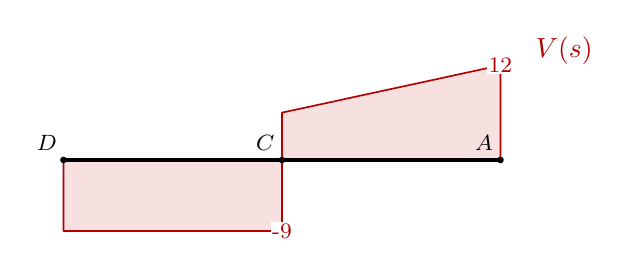
\begin{tikzpicture}[scale=0.925,line join=round]
  \filldraw[fill=red!70!black!12,draw=red!70!black,semithick] (0.000,1.300) -- (-0.125,1.273) -- (-0.250,1.246) -- (-0.375,1.219) -- (-0.500,1.192) -- (-0.625,1.165) -- (-0.750,1.137) -- (-0.875,1.110) -- (-1.000,1.083) -- (-1.125,1.056) -- (-1.250,1.029) -- (-1.375,1.002) -- (-1.500,0.975) -- (-1.625,0.948) -- (-1.750,0.921) -- (-1.875,0.894) -- (-2.000,0.867) -- (-2.125,0.840) -- (-2.250,0.812) -- (-2.375,0.785) -- (-2.500,0.758) -- (-2.625,0.731) -- (-2.750,0.704) -- (-2.875,0.677) -- (-3.000,0.650) -- (-3.000,-0.975) -- (-3.125,-0.975) -- (-3.250,-0.975) -- (-3.375,-0.975) -- (-3.500,-0.975) -- (-3.625,-0.975) -- (-3.750,-0.975) -- (-3.875,-0.975) -- (-4.000,-0.975) -- (-4.125,-0.975) -- (-4.250,-0.975) -- (-4.375,-0.975) -- (-4.500,-0.975) -- (-4.625,-0.975) -- (-4.750,-0.975) -- (-4.875,-0.975) -- (-5.000,-0.975) -- (-5.125,-0.975) -- (-5.250,-0.975) -- (-5.375,-0.975) -- (-5.500,-0.975) -- (-5.625,-0.975) -- (-5.750,-0.975) -- (-5.875,-0.975) -- (-6.000,-0.975) -- (-6.000,0.000) -- (-5.875,0.000) -- (-5.750,0.000) -- (-5.625,0.000) -- (-5.500,0.000) -- (-5.375,0.000) -- (-5.250,0.000) -- (-5.125,0.000) -- (-5.000,0.000) -- (-4.875,0.000) -- (-4.750,0.000) -- (-4.625,0.000) -- (-4.500,0.000) -- (-4.375,0.000) -- (-4.250,0.000) -- (-4.125,0.000) -- (-4.000,0.000) -- (-3.875,0.000) -- (-3.750,0.000) -- (-3.625,0.000) -- (-3.500,0.000) -- (-3.375,0.000) -- (-3.250,0.000) -- (-3.125,0.000) -- (-3.000,0.000) -- (-3.000,0.000) -- (-2.875,0.000) -- (-2.750,0.000) -- (-2.625,0.000) -- (-2.500,0.000) -- (-2.375,0.000) -- (-2.250,0.000) -- (-2.125,0.000) -- (-2.000,0.000) -- (-1.875,0.000) -- (-1.750,0.000) -- (-1.625,0.000) -- (-1.500,0.000) -- (-1.375,0.000) -- (-1.250,0.000) -- (-1.125,0.000) -- (-1.000,0.000) -- (-0.875,0.000) -- (-0.750,0.000) -- (-0.625,0.000) -- (-0.500,0.000) -- (-0.375,0.000) -- (-0.250,0.000) -- (-0.125,0.000) -- (0.000,0.000) -- cycle;
  \draw[line width=1.6pt] (0.000,0.000) -- (-3.000,0.000) -- (-6.000,0.000);
  \node[red!70!black,font=\footnotesize,fill=white,inner sep=0.5pt] at (0.000,1.300) {12};
  \node[red!70!black,font=\footnotesize,fill=white,inner sep=0.5pt] at (-3.000,-0.975) {-9};
  \fill (0.000,0.000) circle (1.3pt);
  \node[font=\footnotesize] at (0.000,0.000) [xshift=-6pt,yshift=6pt] {$A$};
  \fill (-3.000,0.000) circle (1.3pt);
  \node[font=\footnotesize] at (-3.000,0.000) [xshift=-6pt,yshift=6pt] {$C$};
  \fill (-6.000,0.000) circle (1.3pt);
  \node[font=\footnotesize] at (-6.000,0.000) [xshift=-6pt,yshift=6pt] {$D$};
  \node[red!70!black,right] at (0.35,1.50) {$V(s)$};
\end{tikzpicture}\\[5pt]
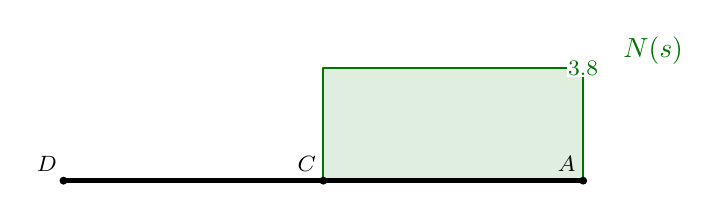
\begin{tikzpicture}[scale=1.100,line join=round]
  \filldraw[fill=green!45!black!12,draw=green!45!black,semithick] (0.000,1.300) -- (-0.125,1.300) -- (-0.250,1.300) -- (-0.375,1.300) -- (-0.500,1.300) -- (-0.625,1.300) -- (-0.750,1.300) -- (-0.875,1.300) -- (-1.000,1.300) -- (-1.125,1.300) -- (-1.250,1.300) -- (-1.375,1.300) -- (-1.500,1.300) -- (-1.625,1.300) -- (-1.750,1.300) -- (-1.875,1.300) -- (-2.000,1.300) -- (-2.125,1.300) -- (-2.250,1.300) -- (-2.375,1.300) -- (-2.500,1.300) -- (-2.625,1.300) -- (-2.750,1.300) -- (-2.875,1.300) -- (-3.000,1.300) -- (-3.000,0.000) -- (-3.125,0.000) -- (-3.250,0.000) -- (-3.375,0.000) -- (-3.500,0.000) -- (-3.625,0.000) -- (-3.750,0.000) -- (-3.875,0.000) -- (-4.000,0.000) -- (-4.125,0.000) -- (-4.250,0.000) -- (-4.375,0.000) -- (-4.500,0.000) -- (-4.625,0.000) -- (-4.750,0.000) -- (-4.875,0.000) -- (-5.000,0.000) -- (-5.125,0.000) -- (-5.250,0.000) -- (-5.375,0.000) -- (-5.500,0.000) -- (-5.625,0.000) -- (-5.750,0.000) -- (-5.875,0.000) -- (-6.000,0.000) -- (-6.000,0.000) -- (-5.875,0.000) -- (-5.750,0.000) -- (-5.625,0.000) -- (-5.500,0.000) -- (-5.375,0.000) -- (-5.250,0.000) -- (-5.125,0.000) -- (-5.000,0.000) -- (-4.875,0.000) -- (-4.750,0.000) -- (-4.625,0.000) -- (-4.500,0.000) -- (-4.375,0.000) -- (-4.250,0.000) -- (-4.125,0.000) -- (-4.000,0.000) -- (-3.875,0.000) -- (-3.750,0.000) -- (-3.625,0.000) -- (-3.500,0.000) -- (-3.375,0.000) -- (-3.250,0.000) -- (-3.125,0.000) -- (-3.000,0.000) -- (-3.000,0.000) -- (-2.875,0.000) -- (-2.750,0.000) -- (-2.625,0.000) -- (-2.500,0.000) -- (-2.375,0.000) -- (-2.250,0.000) -- (-2.125,0.000) -- (-2.000,0.000) -- (-1.875,0.000) -- (-1.750,0.000) -- (-1.625,0.000) -- (-1.500,0.000) -- (-1.375,0.000) -- (-1.250,0.000) -- (-1.125,0.000) -- (-1.000,0.000) -- (-0.875,0.000) -- (-0.750,0.000) -- (-0.625,0.000) -- (-0.500,0.000) -- (-0.375,0.000) -- (-0.250,0.000) -- (-0.125,0.000) -- (0.000,0.000) -- cycle;
  \draw[line width=1.6pt] (0.000,0.000) -- (-3.000,0.000) -- (-6.000,0.000);
  \node[green!45!black,font=\footnotesize,fill=white,inner sep=0.5pt] at (0.000,1.300) {3.8};
  \fill (0.000,0.000) circle (1.3pt);
  \node[font=\footnotesize] at (0.000,0.000) [xshift=-6pt,yshift=6pt] {$A$};
  \fill (-3.000,0.000) circle (1.3pt);
  \node[font=\footnotesize] at (-3.000,0.000) [xshift=-6pt,yshift=6pt] {$C$};
  \fill (-6.000,0.000) circle (1.3pt);
  \node[font=\footnotesize] at (-6.000,0.000) [xshift=-6pt,yshift=6pt] {$D$};
  \node[green!45!black,right] at (0.35,1.50) {$N(s)$};
\end{tikzpicture}\\[10pt]
\end{center}
\end{document}